\providecommand{\main}{..}
\documentclass[\main/tesi.tex]{subfiles}
\begin{document}
\chapter{Strumenti}
\addcontentsline{toc}{chapter}{Strumenti}

In questa sezione verranno illustrati gli strumenti pratici utilizzati per lo sviluppo. \\
La scelta degli strumenti è stata condizionata dall'obiettivo da raggiungere e dal campo di applicazione dell'algoritmo stesso.
Il progetto è stato scritto in F\# \cite{fsharp} in quanto linguaggio creato con lo scopo di essere utilizzato in ambiti logici e matematici data la sua praticità nello sviluppo di tipi e modelli necessari per la creazione di algoritmi dimostrativi. \\
Inoltre il fatto di essere un linguaggio funzionale e la sua sintassi hanno permesso di definire le funzioni ed i modelli con un quantitativo contenuto di linee di codice, specialmente se confrontato con linguaggi orientati ad oggetti. \\

\section{Ecosistema e linguaggi}
\subsection{.NET}
.NET è un ecosistema di sviluppo software creato da Microsoft negli anni 2000 come alternativa a Java. Si basa su un runtime che esegue un bytecode intermedio chiamato \textbf{CIL} \cite{cil} attraverso una macchina virtuale o un compilatore Just in Time.\\
Questo tipo di implementazione consente il supporto a multipli linguaggi di programmazione interoperabili tra di loro (con l'unico vincolo di essere compilabili in CIL) che possono essere eseguiti su qualsiasi sistema operativo per il quale esista una versione del runtime.

Fino al 2015, ufficialmente questo ecosistema era utilizzabile solo su Windows (sotto il nome di .NET Framework \cite{dotnet}), ma in seguito Microsoft sviluppò e rese open source una nuova versione, chiamata .NET Core, più veloce e moderna ma soprattutto multipiattaforma. \\
La versione di .NET \cite{dotnet} utilizzata è la 7.0, l'ultima disponibile, che comporta migliorie rispetto alla 6.0 in termini di:
\begin{itemize}
    \item Prestazioni
    \item Operazioni matematiche
    \item Serializzazione JSON
    \item Espressioni regolari (\textit{Regex})
    \item Osservabilità: Migliora la comprensione dello stato dell'applicazione in base alla scalabilità e come aumenta la complessità tecnica.
    \item SDK: Migliora l'esperienza di utilizzo della \textit{CLI} e consente la gestione e pubblicazione dei pacchetti \textit{nuget} \cite{nuget}
    \item Modelli: Principalmente miglioramenti relativi all'utilizzo del comando \textit{dotnet new} utilizzabile da riga di comando usando la .NET \textit{CLI} \cite{dotnet}
    \item Librerie: Miglioramenti alle librerie di .NET \cite{dotnet}
\end{itemize}
Il progetto in questione è un progetto .NET 7.0 Console \cite{dotnet}. \\

\begin{figure}[h]
    \caption{Funzionamento del .NET runtime \cite{dotnet}, dal web.}
    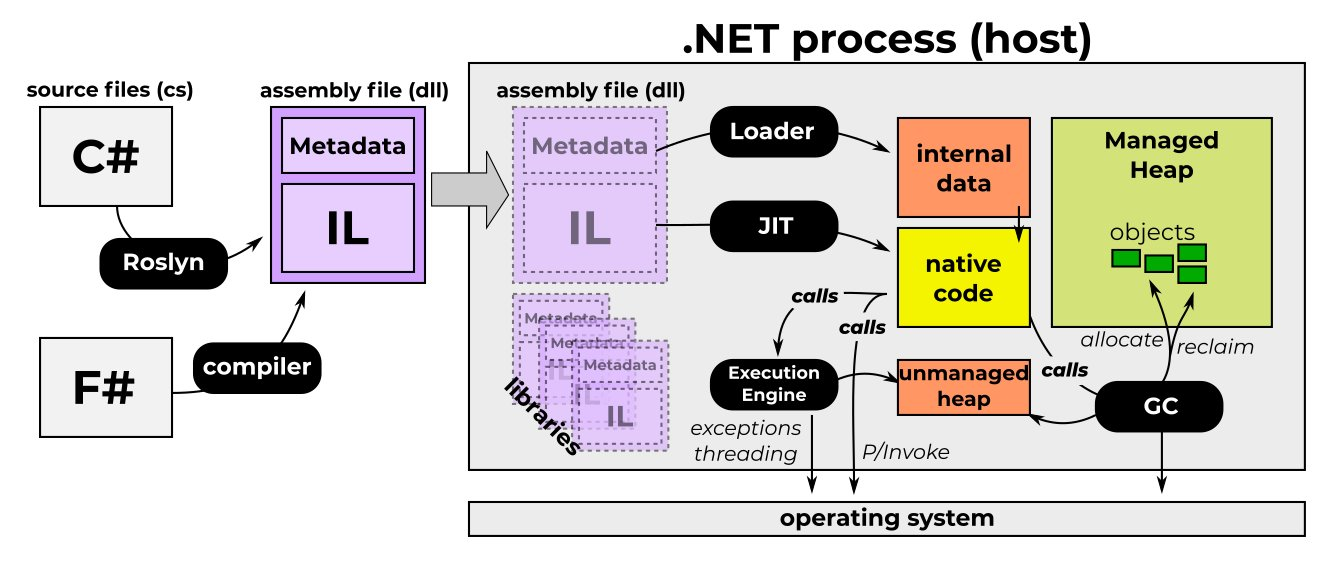
\includegraphics[width=\textwidth]{../images/dotnet.png}
\end{figure}

\newpage

\subsection{F\#}
F\# \cite{fsharp} è un linguaggio di programmazione .NET \cite{dotnet} universale per la scrittura di codice succinto, robusto e performante. \\
Consente di scrivere codice autodocumentato ed è open source e multipiattaforma. \\
Include numerose funzionalità, quali:
\begin{itemize}
    \item Sintassi leggera.
    \item Non modificabile per impostazione predefinita.
    \item Inferenza dei tipi e generalizzazione automatica.
    \item Funzioni di prima classe.
    \item Tipi di dati avanzati.
    \item Criteri di ricerca.
    \item Programmazione asincrona.
\end{itemize}
La versione utilizzata per lo sviluppo è la \textit{7.0}, l'ultima disponibile.

\section{Strumenti di sviluppo}

\subsection{IDE e Text Editors}
L'IDE utilizzato per lo sviluppo è \textit{Visual Studio Code} \cite{vscode}, con l'ausilio di una estensione chiamata \textit{Ionide F\#}. \\
La creazione del progetto e l'installazione dei pacchetti \textit{nuget} \cite{nuget} necessari è avvenuta tramite l'utilizzo della .NET CLI mediante il comando \textit{dotnet new}. \\
L'utilizzo di questo editor è motivato dal fatto che si tratta del più famoso ed utilizzato, ma il progetto è compatibile anche con 'IDE \textbf{Visual Studio} \cite{visualstudio} in quanto verrebbe interpretato come una \textit{Console Application}. \\

\subsection{Nuget Package Manager}
\textbf{Nuget} \cite{nuget} è il nome del più popolare package manager utilizzato nel mondo .NET \cite{dotnet}.\\
E' stato utilizzato per la gestione dei pacchetti pubblici forniti da Microsoft o terze parti (contenuti nel repository principale residente in nuget.org).\\
Nuget consente infatti la creazione di pacchetti da salvare in un server locale o HTTP, per essere consumati da qualsiasi progetto, semplificando la condivisione di librerie.\\

\subsection{Versioning e Task Management}
Nello sviluppo software, gli strumenti di versioning sono vitali per la gestione di progetti complessi.
Permettono infatti di sincronizzare il lavoro di multipli sviluppatori sullo stesso codice.\\
Ma è anche necessario tenere traccia di bug, feature e versioni.\\
Il sistema utilizzato per soddisfare questi requisiti è \textbf{GitHub} \cite{github}.\\

\end{document}